\documentclass{notube}
\usepackage{capt-of}
\usepackage{url}
\makeatletter
\g@addto@macro{\UrlBreaks}{\UrlOrds}
\makeatother
\usepackage{subfig}

\WP{7c} \WPName{Internet TV in the Social Web}

\delID{7c.4} \delName{Social TV Integrated Prototype of v.1 and v.2}
\delNameRunning{Deliverable D7c.4} \delCoordinators{Libby Miller (BBC)}

\delContributors{Vicky Buser (BBC), Dan Brickley (VU)}

\delQualityAssessor{Luca Vignaroli}

\delQualityController{Lyndon Nixon}

\dueContractual{M33}
\dueActual{31-10-11}
\status{1.0}

%\final

%\prototype
\report
%\dissemination

\public
%\consortium

\authorPartner{Libby Miller (BBC),  Vicky Buser (BBC),  Dan Brickley (VU)}
\responsibleAuthor{Libby Miller (BBC)}
\responsibleAuthorPartner{BBC}
\responsibleAuthorEmail{libby.miller@bbc.co.uk}
\responsibleAuthorPhone{+44 (787) 6565561}

\summary{
This document summarises the work done so far in the workpackage `TV and the Social web' (WP7c). It describes the approach we have taken, the prototypes we have made, and our plans for the final three months of the project.
}

\abstract{
In the workpackage `TV and the Social web' (WP7c) we have used lightweight prototyping techniques in order to explore social TV in on-demand, live TV, and second screen authoring evironments, using multiple connected screens. We have gone significantly beyond the state of the art by creating standards-based prototypes that allow small and large groups to collaborate and interact in real time while watching TV or finding interesting things to watch and share. 
We argue that using metadata as an advert for TV programmes, unique URLs for TV, and device independent APIs to TV and TV-like devices make second screen applications significantly more useful and interesting. 
}

\keywords{TV, television, set top box, media centre, iphone, ipad, XMPP, jabber, \\
strophe, voting, companion device, second screen, authoring tools,\\ 
HTML5
}

\versionLog{
    \versionLogEntry{\today}{Libby Miller}{1.0}
}


\begin{document}

\maketitle

%\include{abbreviations}

\chapter{Introduction}

\section{Deliverable Objective}

The aim of this deliverable, D7c.4, is to:
\begin{itemize}
\item{Describe the approach we have taken throughout the project}
\item{Summarise the work we have done so far}
\item{Describe the principles behind the work}
\item{Describe the results}
\item{Describe our plans for the final months}
\end{itemize}


\section{Approach}

We defined our approach in our first deliverable, summarising the text of the proposal about this part of the project, which had become outdated :

\begin{itemize}
\item{Enhance TV user experience by helping users find content they enjoy by making TV more social}
\end{itemize}

by

\begin{itemize}
\item{Being able to flexibly and quickly demonstrate ideas in a compelling fashion}
\item{Allowing users to share information and recommendations and create textual user generated content - essentially metadata about television - using appropriate social media tools}
\item{Enabling users to share their profile information while respecting user privacy}
\item{Testing the result with BBC content}
\end{itemize}

\noindent Two things became clear early on in this project:

\begin{itemize}
\item{Social media and TV was and continues to be a very fast-moving area, and our ideas were in danger of being overtaken by commercial projects}
\item{Second screens were the model of interaction that was both obvious and increasing in popularity}
\end{itemize}

The first issue meant that it was very important for us to be very flexible, and also to try to think beyond the obvious connections between social media and TV around Twitter and Facebook (i.e. not just `Tweet this to your friends'). 

The second issue threw up our biggest problem: designing for second screens for TV requires overcoming the lack of two-way communication between most TVs and any other devices. Most consumer-orientated TVs and TV-like devices currently have nothing like this, which means no simple or direct way of synchronising the second screen device and the TV. 

This deliverable is about how we chose some obvious problems viewers have, and tried to solve them using ideas that are a step further than what is commercially being produced, but using technology that largely already exists. 



\chapter{What have we built?}

We have made prototypes in three main areas:

\begin{itemize}
\item{Live TV Companion}
\item{On-demand browsing}
\item{Authoring second screen content}
\end{itemize}


\section{Live TV Companion}

The basis of our first prototype was: `Do you want to know more?', a reference to the film `Starship Troopers' in which each news item ends with various options for further related exploration, producing the possibility of a non-linear exploration through the available content. We wanted to create the means for viewers to explore what they are watching more deeply using a connected second screen. This type of exploration is a very common reason for using a non-connected second screen while watching TV\footnote{See \url{http://www.lostremote.com/2011/10/13/what-tv-viewers-are-doing-on-their-tablets-smartphones/} and  \url{http://ovum.com/2011/10/04/unlocking-the-second-screen/}}. Our view was that if this could be automated or part-automated, there would be many opportunities for making television more interactive and informative, and also more social. The social aspect of TV watching comes from talking about the programme: opinions but also facts, connections and referencing related material on the Web. You can see the usecase illustration in Figure \ref{fig:more}. 

\begin{figure}[htbp]
\begin{center}
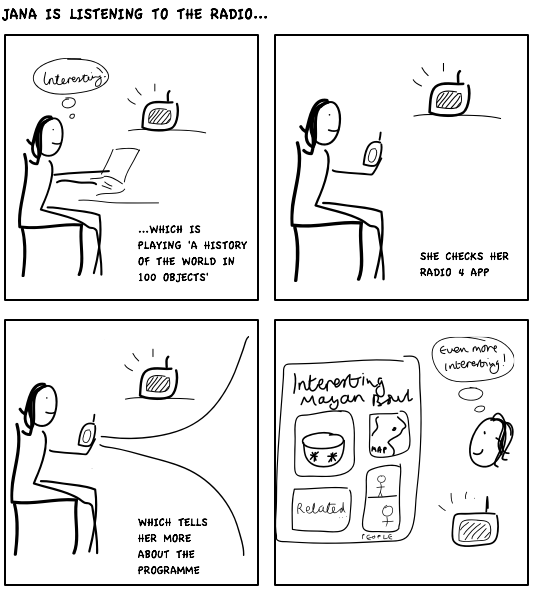
\includegraphics[width=6in]{images/more.png}
\caption{Usecase: Do you want to know more?} \label{fig:more}
\end{center}
\end{figure} 

Our goal was to use unique programme identification, combined with NoTube services, coupled with a connection to the TV, to produce relevant and interesting information about the programme being viewed, which could then be explored on a second screen, and shared. This turned out to be more difficult than we expected.

It was clear even at this early point in the project that second screens were the most appropriate mechanism from a user experience point of view for exploring programmes more deeply, including more socially. However, typically, consumer-orientated TVs and TV-like devices such as PVRs (Personal Video Recorders) only have one external-developer-accessible control interface, which is the infra-red remote control. For our prototype to work we needed both to be able to control the TV and also to be able to identify what programme was showing on the TV. In the past year this problem of synchronisation of screens has been tackled using work-arounds such as audio-watermarking\footnote{For example \url{http://www.bbc.co.uk/blogs/researchanddevelopment/2011/09/orchestrated-media-based-tv--.shtml}}. We took a more direct approach, and identified a TV software platform that we could develop with, which also had control and feedback APIs accessible to the more casual developer.

Our first prototype was therefore a second screen application that worked with MythTV, an open source software TV receiver, to display information related to the programme. Instead of being specifically designed for any particular platform, we designed an API (`Buttons') to generalise over multiple devices and applications. We created a native iPhone application in order to use the device's capabilities for discovery of available TV devices. The underlying synchronisation platform was XMPP (Extensible Messaging and Presence Protocol), an XML messaging framework with identity, contact and group management. 

\begin{figure}[htbp]
\begin{center}
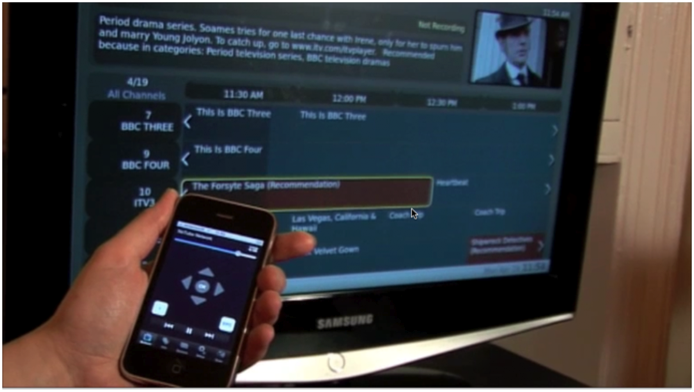
\includegraphics[width=6in]{images/year1.png}
\caption{Live TV Companion in action} \label{fig:year1}
\end{center}
\end{figure} 

From this prototype we learned several things:

\begin{itemize}
\item{It is difficult to automate finding content related to a particular programme, and although unique identification of a programme takes place in the production of metadata, this identification is not made available in a useful form to end users. In order to be able to present the user with interesting information about the programme they are watching it needs to be specific to that programme, and not about another programme from the same series, or about the series itself, or about something else which happens to have the same name.}
\item{XMPP is a promising technology for syncing between devices, allowing us to punch through firewalls (enabling usecases like `record this programme for me at home when I'm at work') and host infrastructure on external servers}
\item{iPhone prototyping is comparatively slow, and (obviously) limits the devices that can be used}
\item{A substantial amount of infrastructure was missing to make social TV real beyond the obvious and already-existing techniques (such as having a `Twitter' or `Facebook' button)}
\end{itemize}

The main piece of infrastructure missing had to do with the specific identification of programmes. We needed the ability to go from the unique `crid' (Content Reference Identifier\footnote{\url{http://en.wikipedia.org/wiki/Content_Reference_Identifier}}) which is broadcast over the air as part of the EIT metadata (Event Information Table\footnote{\url{http://en.wikipedia.org/wiki/Program_and_System_Information_Protocol}}) to information that people could read or share. Heavily inspired by RadioDNS\footnote{\url{http://radiodns.org/}}, and collaborating with Mo McRoberts of Project Baird\footnote{\url{http://projectbaird.com/discovery/tvdns/}}, we wrote a resolver for BBC programmes that takes a crid and returns the unique BBC URL for the programme and vice-versa\footnote{\url{http://notube.tv/2010/08/26/connecting-broadcast-tv-and-the-web-using-a-resolver/}}, bridging the gap between the two worlds in the sense that if you have a BBC programmes URL and a DVB player you can play the video on it; and if you have the crid and the Web you can find out more about it, and share that link with others in social media.

In order to be able to create prototypes quickly, after the first year we moved to HTML / Javascript using an XMPP backend infrastructure and APIs on top of that. We built some of the infrastructure we needed and tried to persuade people in the industry of the importance of URLs for programmes for social web communication, metadata as an advert for content, and the usefulness of APIs to TV.\footnote{\url{http://www.w3.org/2010/11/web-and-tv/papers/webtv2_submission_60.pdf}}

Although we have created other prototypes to be used with live TV (for example, an application to allow real-time voting and visualisation of votes\footnote{\url{http://jabber.notu.be/thekilling/}}, Figure \ref{fig:votey}), and an autocompleting twitter API for TV\footnote{\url{http://notube.tv/2010/11/22/epg-autocompleter/}}, most effort after this period has been spent on considering the various problems of on-demand content, particularly the problem of choice within large corpuses of content. There are a number of interesting problems in this area, particularly as the number of on-demand videos is growing very rapidly\footnote{\url{http://www.cisco.com/en/US/solutions/collateral/ns341/ns525/ns537/ns705/ns827/white_paper_c11-481360_ns827_Networking_Solutions_White_Paper.html}}. This decision was also taken because of the problems we had creating reliable and sustainable demonstrators using the MythTV setup and the lack of alternatives for playing live TV, and that we could not make much more interesting progress in this area.


\begin{figure}[htbp]
\begin{center}
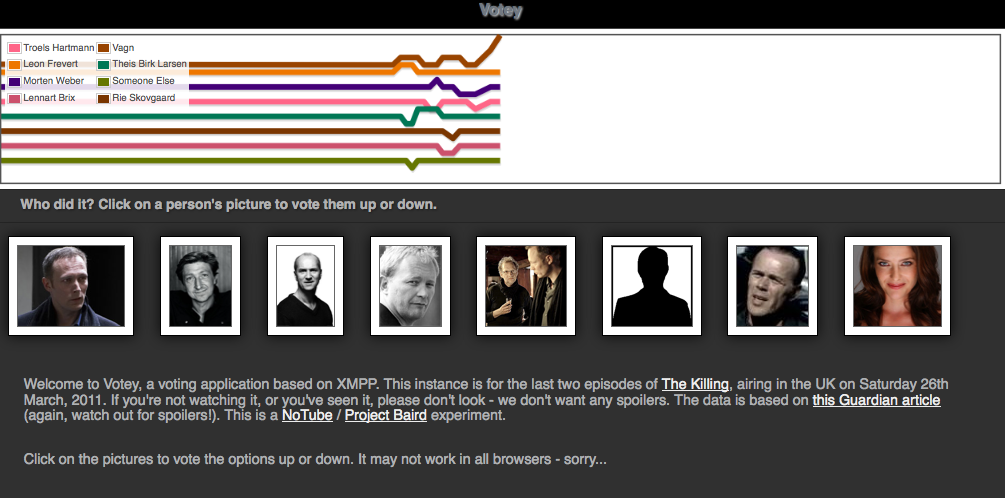
\includegraphics[width=6in]{images/votey.png}
\caption{`Votey' - Real-time graphing of votes} \label{fig:votey}
\end{center}
\end{figure} 

\section{On-Demand Prototypes}

We have made two main prototypes in the on-demand area, both centred around problems of choice. When faced with a large number of potential options, many people find it difficult to choose, and give up quickly\footnote{see \url{http://flowtv.org/2010/10/choice-fatigue-community-and-the-mutations-of-television/} and \url{http://en.wikipedia.org/wiki/Least_objectionable_program}}. For video content owners this means that much of their content may never get the attention of people who are interested in it, either directly, or via social media sharing.

The first prototype (`Archive Browser') was designed to test whether presenting related content could make people browse longer. The second one (`N-Screen') attempts to harness the `look what I found' impulse for the same purpose.

Both of these applications are Web-based, and can be used as second screen applications, with another web-page acting as the `TV'.

\subsection{Archive Browser}

The Archive Browser addresses the usecase of finding something interesting to watch later. It could be applicable to any on-demand archive, for example BBC's iPlayer system. It's illustrated in Figure \ref{fig:archive}.

\begin{figure}[htbp]
\begin{center}
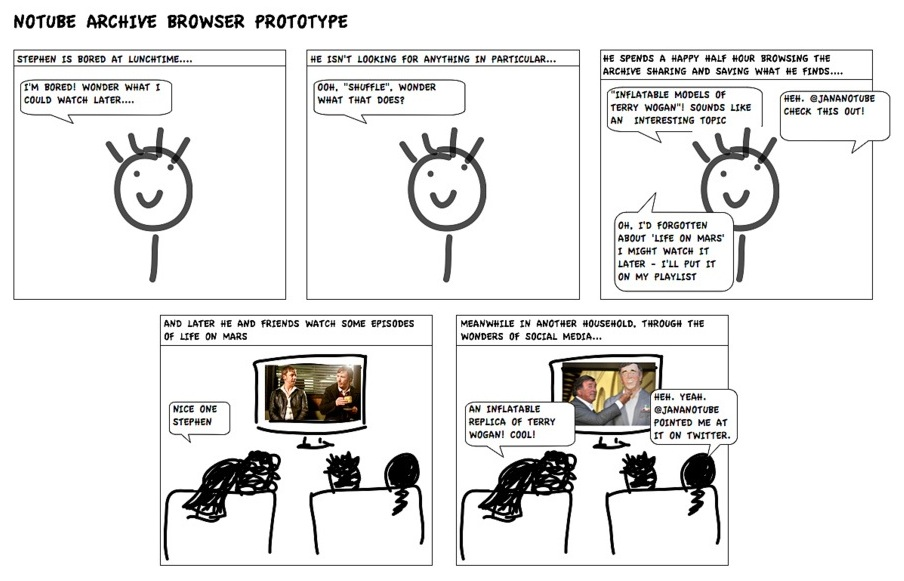
\includegraphics[width=6in]{images/archive.jpg}
\caption{Usecase: Finding a programme to watch later} \label{fig:archive}
\end{center}
\end{figure} 


This particular version is an HTML-based browser of a subset of BBC's Redux project\footnote{\url{http://www.bbc.co.uk/blogs/bbcinternet/2008/10/history_of_the_bbc_redux_proje.html}}. We designed it to test experimentally whether people spent more time browsing and adding to a playlist if related content was presented to them in a randomised trial using 90 volunteers from within the BBC. The results were inconclusive, although people liked the approach whichever group they were placed in -  but one interesting thing did emerge: people like having a `random' (or `shuffle') button\footnote{\url{http://notube.tv/2011/07/01/finding-interesting-new-programmes-trial-results/}}. We also made the data for this experiment open for others to download and use\footnote{\url{http://notube.tv/2011/02/15/linking-wikipedia-and-bbc-programmes/}}. We were also able to combine this prototype with the kt Korlex Korean Wordnet using mappings between the BBC's classifications system, Lonclass\footnote{\url{http://en.wikipedia.org/wiki/Lonclass}}, in order to be able to search and browse the subset of this archive in Korean (see Figure \ref{fig:korlex}).

\begin{figure}[htbp]
\begin{center}
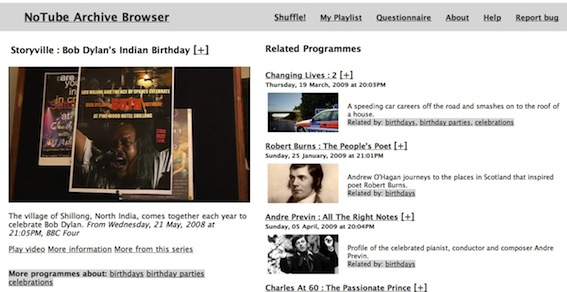
\includegraphics[width=6in]{images/notube-archive-browser.jpg}
\caption{NoTube Archive Browser} \label{fig:archive}
\end{center}
\end{figure} 

\begin{figure}[htbp]
\begin{center}
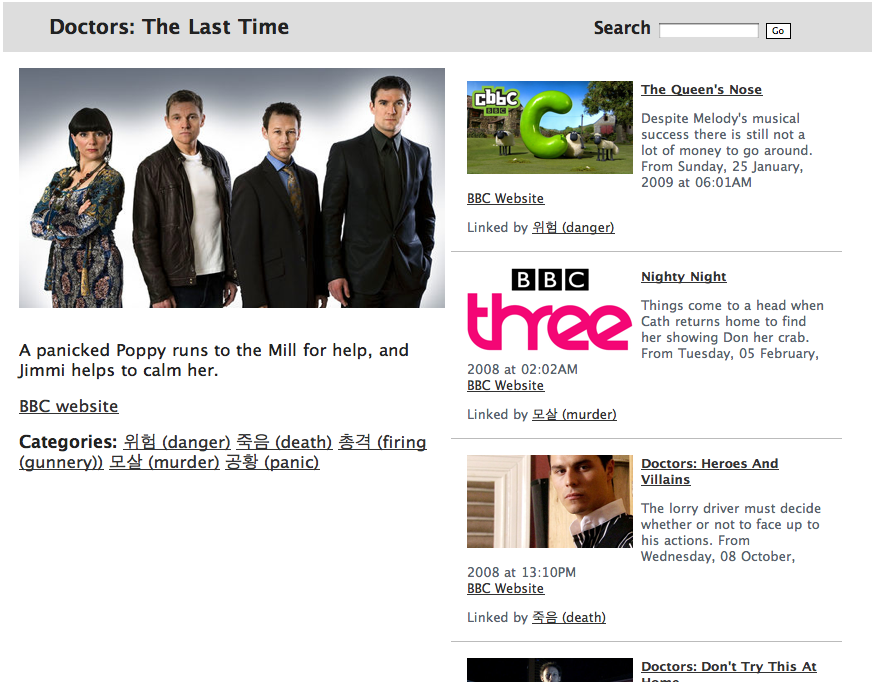
\includegraphics[width=5in]{images/korlex.png}
\caption{NoTube Archive Browser with Korean categories} \label{fig:korlex}
\end{center}
\end{figure} 

\subsection{`N-Screen'}

N-Screen explicitly addresses issues of choice in a social situation. Because people have preferences about each others' mental states as well as their own (i.e. they make decisions based on whether the other person will also enjoy a programme), choosing in small groups can be very difficult. The usecase is illustrated in Figure \ref{fig:nscreen_usecase}.

\begin{figure}[htbp]
\begin{center}
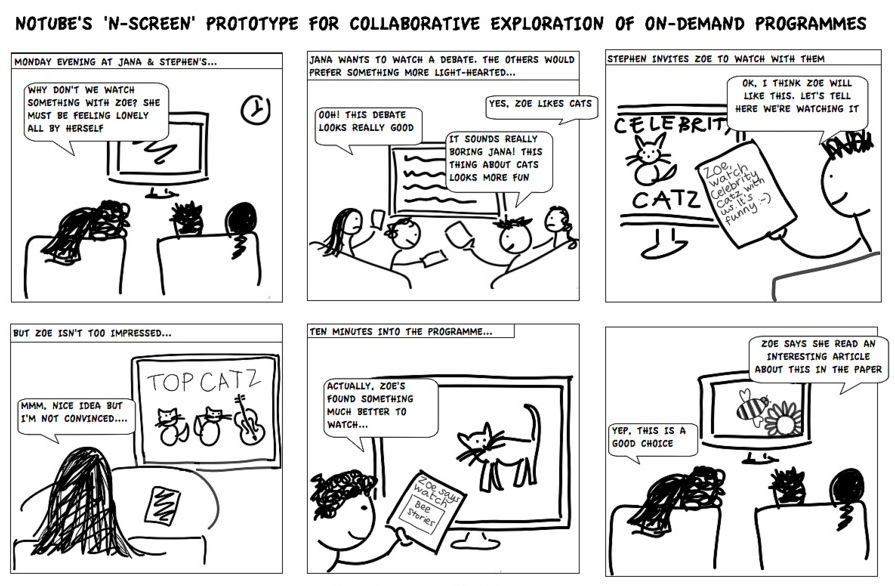
\includegraphics[width=5in]{images/nscreen_usecase.jpg}
\caption{Usecase: Finding things to watch in small groups} \label{fig:nscreen_usecase}
\end{center}
\end{figure} 

N-Screen is a second screen HTML / Javascript application that allows people to express their preferences to each other directly, by dragging and dropping items to each other individually or as a group. Group members can be in the same room or physically distant, and one or more TVs can be synced to watch together remotely. It is primarily for tablets and laptops, but runs on anything with a modern Web browser; from smartphones to touch-tables and desktop PCs. It is designed for multiple screens in use while watching TV, explicitly addressing the `second screen' issues (but taking it a logical step further), but also some of the social aspects of TV watching, ones that we believe have not been addressed elsewhere. We are also interested in, but have not yet tested, whether people will spend longer browsing when they have the opportunity to share what they have found with others.

We have made three different version of N-Screen with three different sets of content: Redux, TED Talks, and iPlayer\footnote{\url{http://notube.tv/2011/10/10/n-screen-a-second-screen-application-for-small-group-exploration-of-on-demand-content/}}, with different approaches to content to content recommendation encapsulated within each, depending on the data available\footnote{\url{http://notube.tv/2011/10/14/algorithms-for-recommendations-in-various-n-screen-implementations/}}. You can see a screenshot in Figure \ref{fig:nscreen}.

We are indebted to the VU for their work in arranging for design help, and to Fabrique\footnote{\url{http://www.fabrique.nl/}} for designs to improve the appearance of N-Screen.

\begin{figure}[htbp]
\begin{center}
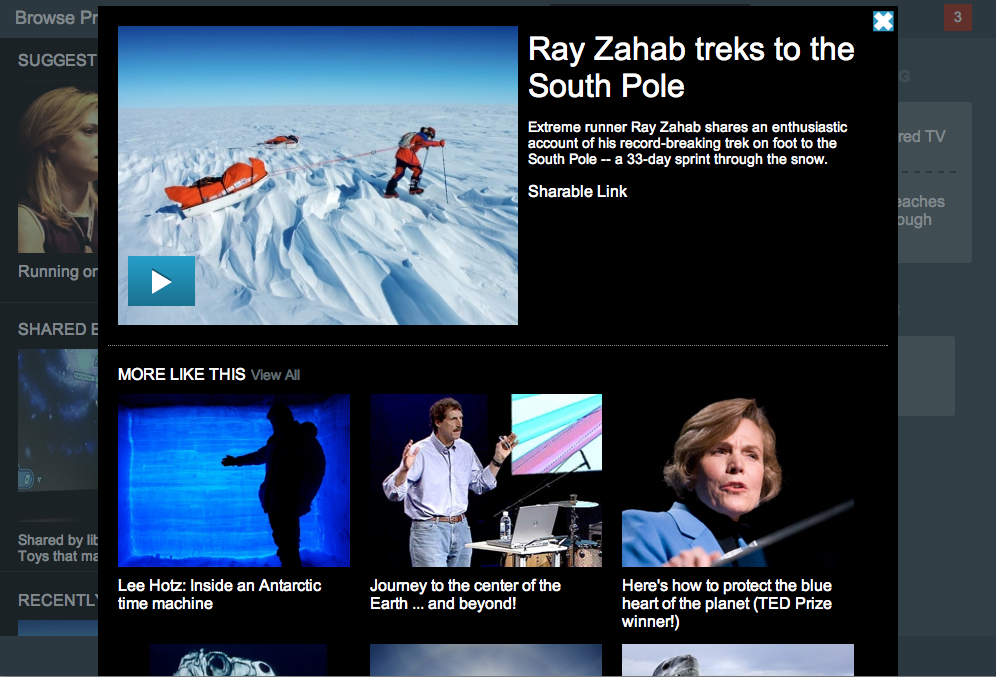
\includegraphics[width=6in]{images/nscreen.png}
\caption{N-Screen - small-group collaborative browsing of video collections} \label{fig:nscreen}
\end{center}
\end{figure} 


\section{Tools for Authoring and Playback of Second Screen Content}

Our final set of demonstrators starts to consider some of the problems with authoring second screen content, and whether collaboration can help. It uses the same infrastructure as N-Screen but shows some of the different ways it can be used.

\subsection{TV Extras Authoring (`TEA')}

TEA lets you author basic extras for the second screen, as you watch a video, using drag and drop from searches of the web. It is a web application built using HTML5. The usecases concern:

\begin{itemize}
\item{Professional, common-place second screen content authoring within organisations}
\item{Enthusiast annotation}
\end{itemize}

Currently we only address on-demand authoring. 

In the application, two or more people can see each others' suggestions for second screen links and review it. Either can then sync the video for playback, so they can review it together. Finally, they can save their work to an intermediate file format for playback on other devices. This intermediate file is in some ways the most interesting part, as it enables expert developers for particular platforms to create second screen playback tools without also having to handle the authoring side.

\begin{figure}[htbp]
\begin{center}
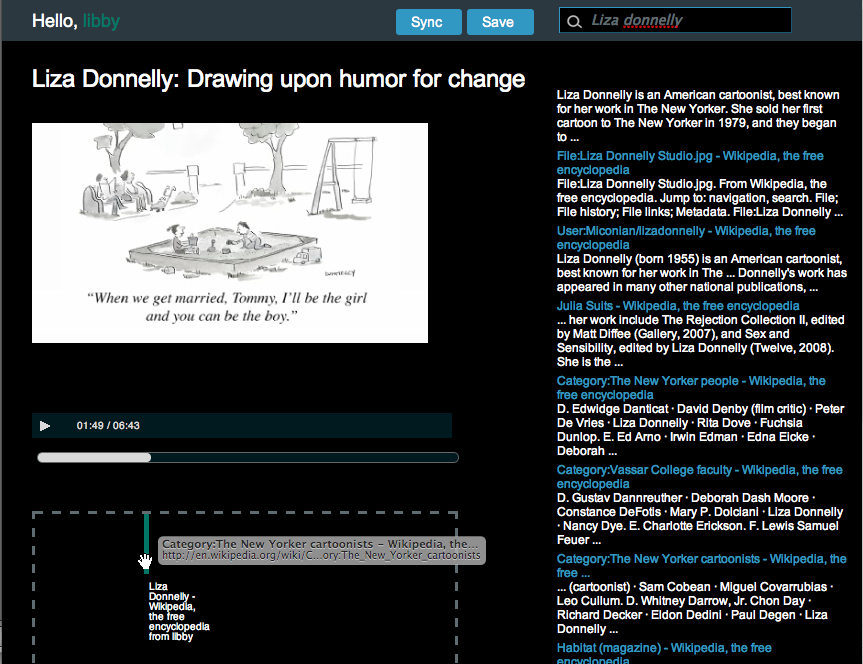
\includegraphics[width=6in]{images/tea.png}
\caption{`TEA' - TV Extras Authoring} \label{fig:tea}
\end{center}
\end{figure} 


\subsection{TEAPlayer}

TEAPlayer is an experimental iPhone application built with Phonegap\footnote{\url{http://www.phonegap.com/}}(so the bulk of it is HTML) to play the output format of TEA on XBMC (XBox Media Centre). The idea was to see if the information in the file format produced using TEA was sufficient to be made into a useful tool. The result is an iPhone application that looks for XBMC (a video player) instances on the same network, and allows the user to choose from a selection of videos on an iPhone to play on it. If she chooses an annotated video, it loads the URLs on the iPhone at the correct time during playback. It also enables her to pause and play the currently playing video - see Figure \ref{fig:teaplayer}.

\begin{figure}
%  \centering
\subfloat[TEAPlayer showing remote functionality]{
  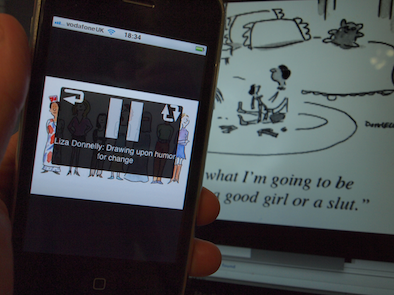
\includegraphics[width=3in]{images/tea_player1.png}
}
\subfloat[TEAPlayer showing link appearing on second screebn]{
  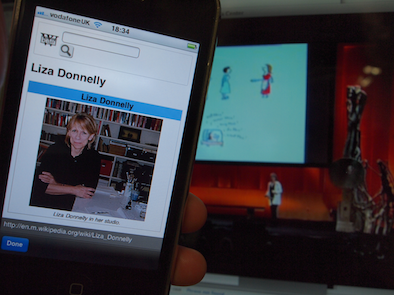
\includegraphics[width=3in]{images/tea_player2.png}
}


  \label{fig:teaplayer}
\end{figure}


\section{Next steps}

In the final three months of the project we want to tackle the following final tasks:

\section{Integration of personalised recommendations}

N-Screen provides the capacity for several different kind of recommendations, including personalised ones from a source such as Beancounter. We are mid-way though a lightweight integration of Beancounter and N-Screen, using Beancounter as a datasource for N-Screen and vice-versa.

\section{Evaluation and user testing}

Two pieces of user testing are planned:

\begin{itemize}
\item{General comparison of second screen and on-screen information}
\item{User evaluation of N-Screen}
\end{itemize}

\section{Refining the TEA file format}

We are researching possible existing formats for describing URL-based annotation at points in a video.

\section{Completing and publishing an implementation of the `Buttons' Javascript API}

This will allow developers to use second screen applications without worrying about the detail of the XMPP infrastructure.


\chapter{What have we learned?}

Our conclusions remain the same as those expressed in February 2011 in our paper to the Web and TV workshop in Berlin (with Mo McRoberts)\footnote{\url{http://www.w3.org/2010/11/web-and-tv/papers/webtv2_submission_60.pdf} (pdf)}. We enumerated the key problems facing developers of second screen content:

\begin{itemize}
\item{(a) How do we know what the person is watching?}
\item{(b) How do we locate additional information about the programme?}
\item{(c) How do we locate apps or Web pages related to it?}
\item{(d) How can we manipulate it?}
\end{itemize}

We proposed three parts of a solution


\section{Use metadata as an advert for the content that can flow out into the public Web in search of viewers}
\section{Create URLs for the content items}

These first two two help social TV discovery, by giving people a Web reference to use and by letting people see something about what they are talking about even if they cannot (or don't feel inclined to) watch it right away.  APIs to see what is playing and identify it, to pause, play and otherwise manipulate a remote TV player enable multiple interesting second screen applications, by enabling synchronisation of second screen content.

\section{Agree on open APIs for controlling the TV and getting access to metadata from it}

As we have gradually realised within the project, the worlds of TV and the Web are far apart in many ways, but particularly important to our work has been the difference between Web developers and TV developers, which can be summarised very crudely as experimentation versus reliability. The Web is a platform that rewards and generates novelty and change. The TV world is largely about making reliable appliances. The specifications in each world are appropriately weighted. The attention spans of the developers are sized proportionately to the specifications. Add to this the concerns of content owners about the accessibility of   their content to non-rights holders - this applies to metadata as well as video - and it is not surprising that control over the device is restricted. In retrospect, making anything that spans these two worlds in any direct sense was going to be difficult.
\\

What is also clear is that if aspects of the TV experience could be made available to web developers, there could be an explosion of related applications for second screens. To harness the creativity of the vast number of web developers, a TV API needs to be extremely easy to use and understandable within a page or two of documentation. This is a very, very different way of working to TV developers, and there is a large chasm of understanding between the two groups. It was very disappointing to see a plethora of `Apps' and APIs to TV at IBC 2011, with no standard in place to mitigate the effect of this diversity on consumers and developers.

We have tried to demonstrate throughout the project that \emph{if} APIs to TV existed, \emph{then} social TV would become more compelling, and created multiple \emph{user-focused} prototypes which (we hope) show this, as well as pursuing standards-based solutions to the problem via W3C's Web and TV Interest Group, and working with the BBC's `UC' API.\footnote{\url{http://www.bbc.co.uk/rd/publications/whitepaper194.shtml}} Throughout, we have tried to use tools and frameworks that allow us to create prototypes as quickly as possible, while using diverse techniques for coming up with interesting and relevant usecases and scenarios.\footnote{\url{http://notube.tv/author/vickybuser/}}. We have documented our approach and technical work as blog posts, photos and video, and by creating a list of links on delicious, and we have worked in public where possible, so that the work will continue to be useful in the future.

\end{document}


%\begin{figure}[htbp]
%\begin{center}
%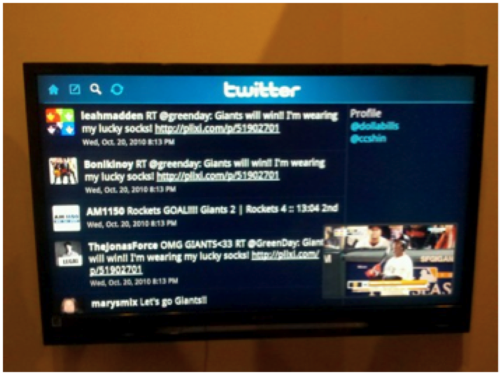
\includegraphics[width=6in]{images/googletv.png}
%\caption{Twitter on GoogleTV} \label{fig:google}
%\end{center}
%\end{figure} 



